
\chapter{Results}

\section{Pipelines}

\subsection{Output}

\begin{figure}[H]
  \centering

  \begin{subfigure}{0.48\textwidth}
    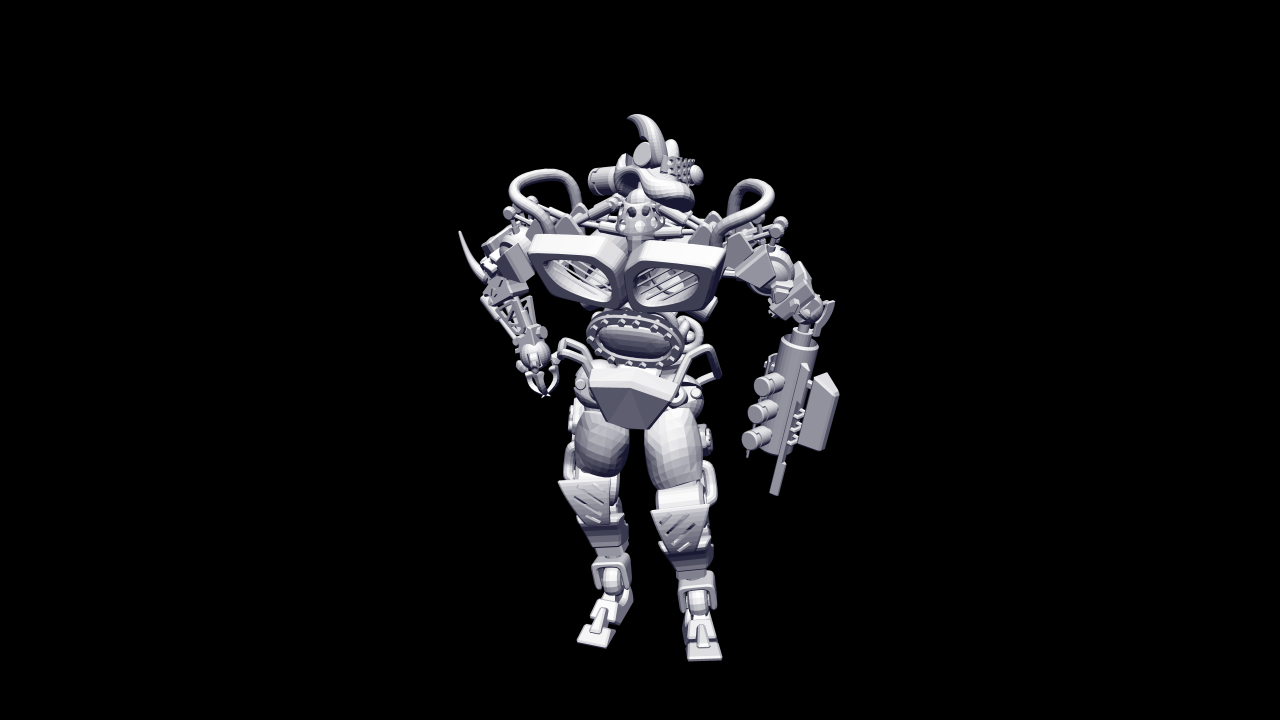
\includegraphics[width=\linewidth]{figures/brainstem_normal.png}
    \caption{Standard pipeline}
  \end{subfigure}\hfill
  \begin{subfigure}{0.48\textwidth}
    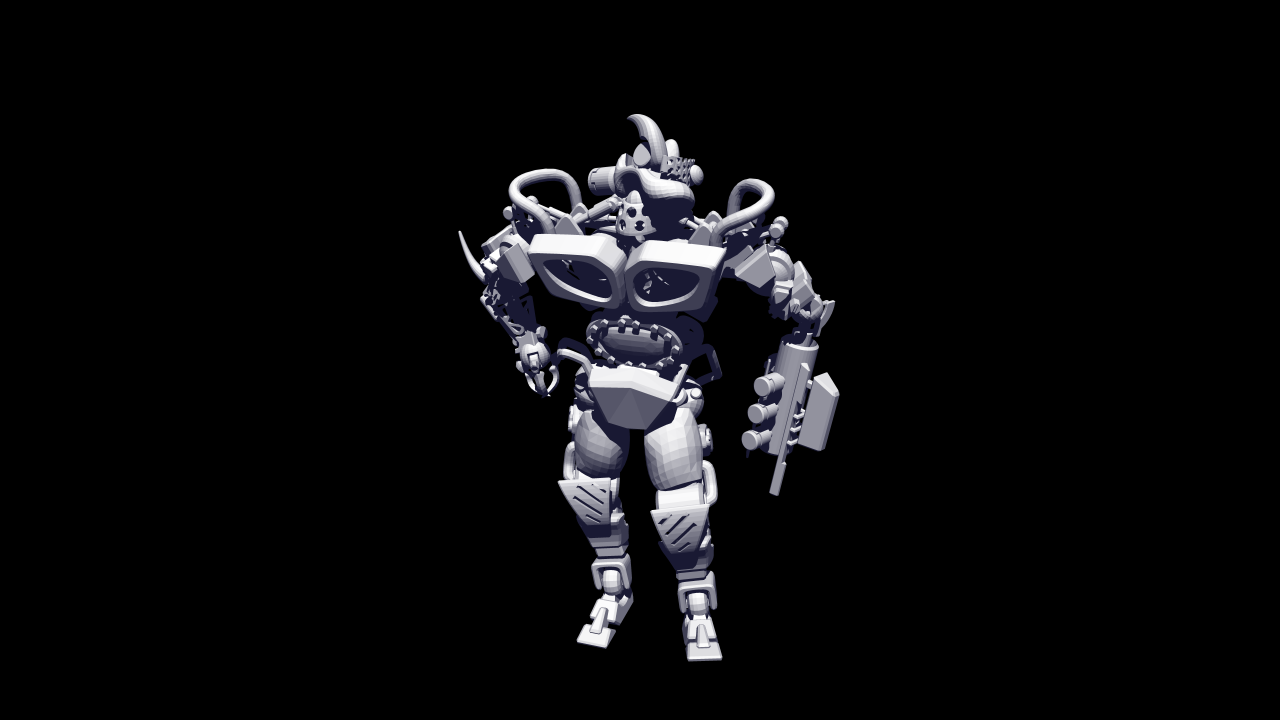
\includegraphics[width=\linewidth]{figures/brainstem_shadow.png}
    \caption{Shadow pipeline}
  \end{subfigure}\hfill
  \begin{subfigure}{0.48\textwidth}
    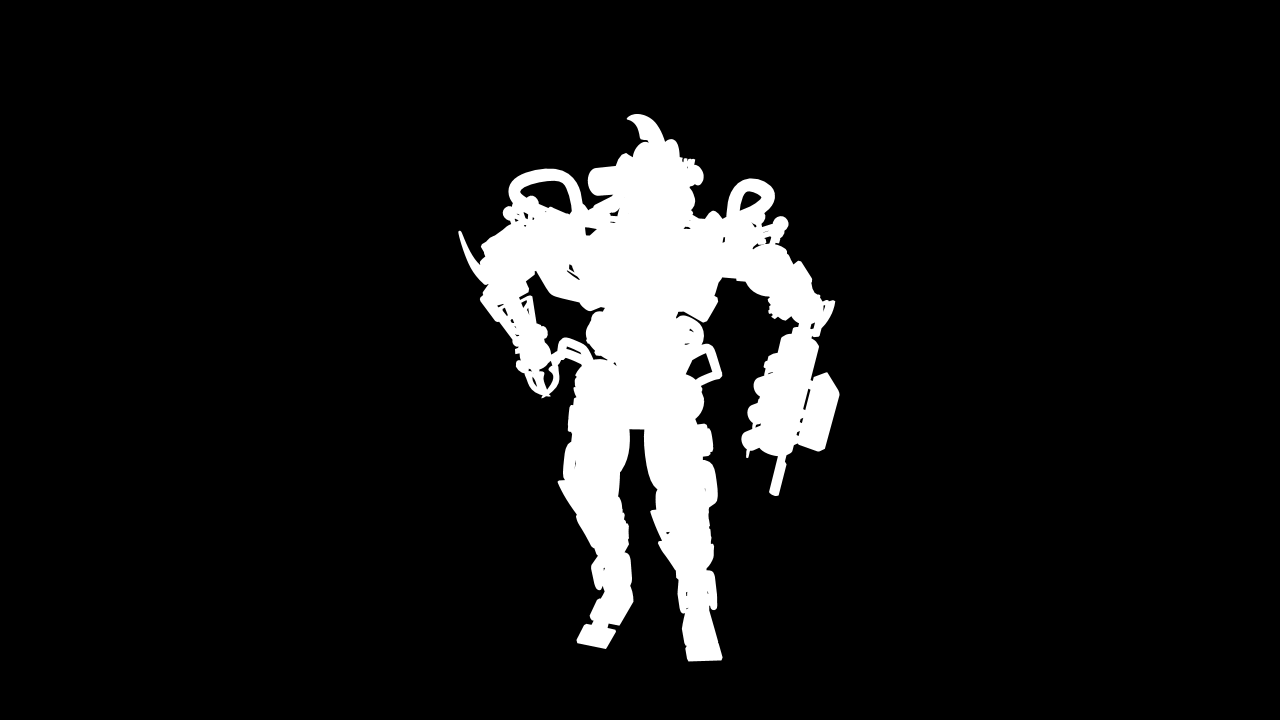
\includegraphics[width=\linewidth]{figures/brainstem_basic.png}
    \caption{Basic pipeline}
  \end{subfigure}

  \caption{Output images using different pipelines for the scene "BrainStem"}
\end{figure}

\begin{figure}[H]
  \centering

  \begin{subfigure}{0.48\textwidth}
    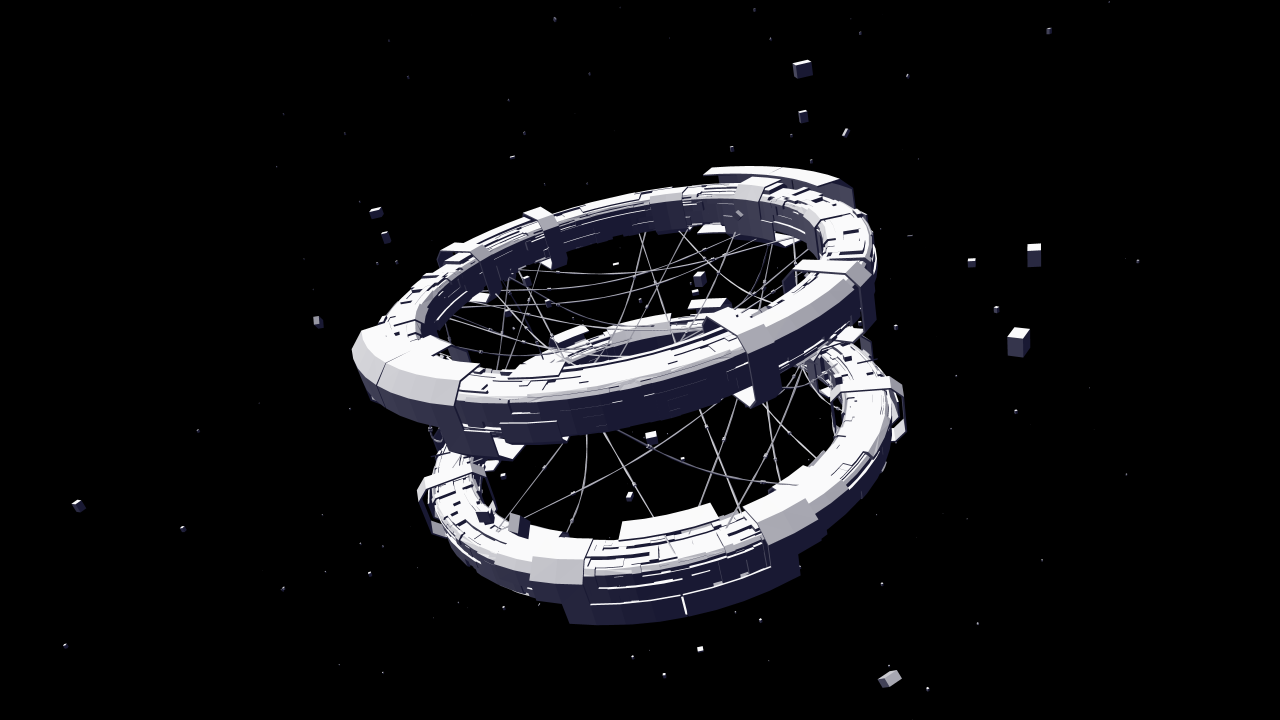
\includegraphics[width=\linewidth]{figures/space_station_normal.png}
    \caption{Standard pipeline}
  \end{subfigure}\hfill
  \begin{subfigure}{0.48\textwidth}
    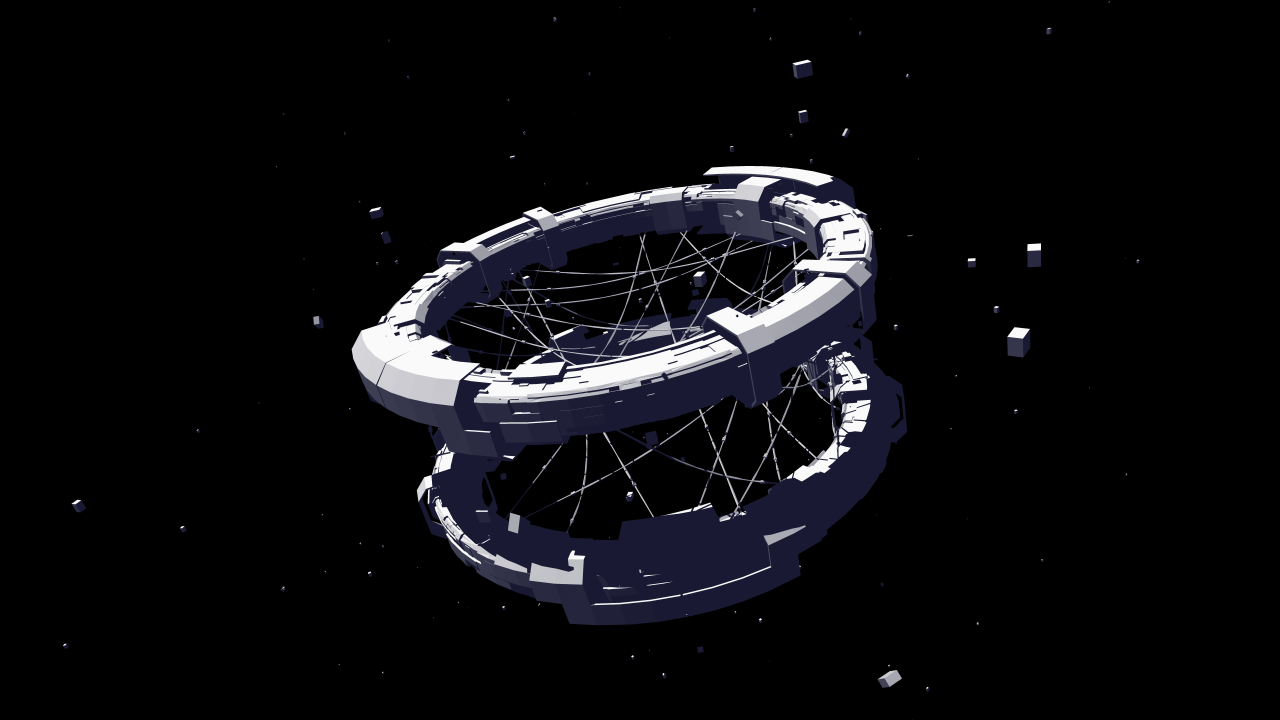
\includegraphics[width=\linewidth]{figures/space_station_shadow.png}
    \caption{Shadow pipeline}
  \end{subfigure}\hfill
  \begin{subfigure}{0.48\textwidth}
    
\includegraphics[width=\linewidth]{figures/space_station_basic.png}
    \caption{Basic pipeline}
  \end{subfigure}

  \caption{Output images using different pipelines for the scene "Space Station"}
\end{figure}

\begin{figure}[H]
  \centering

  \begin{subfigure}{0.48\textwidth}
    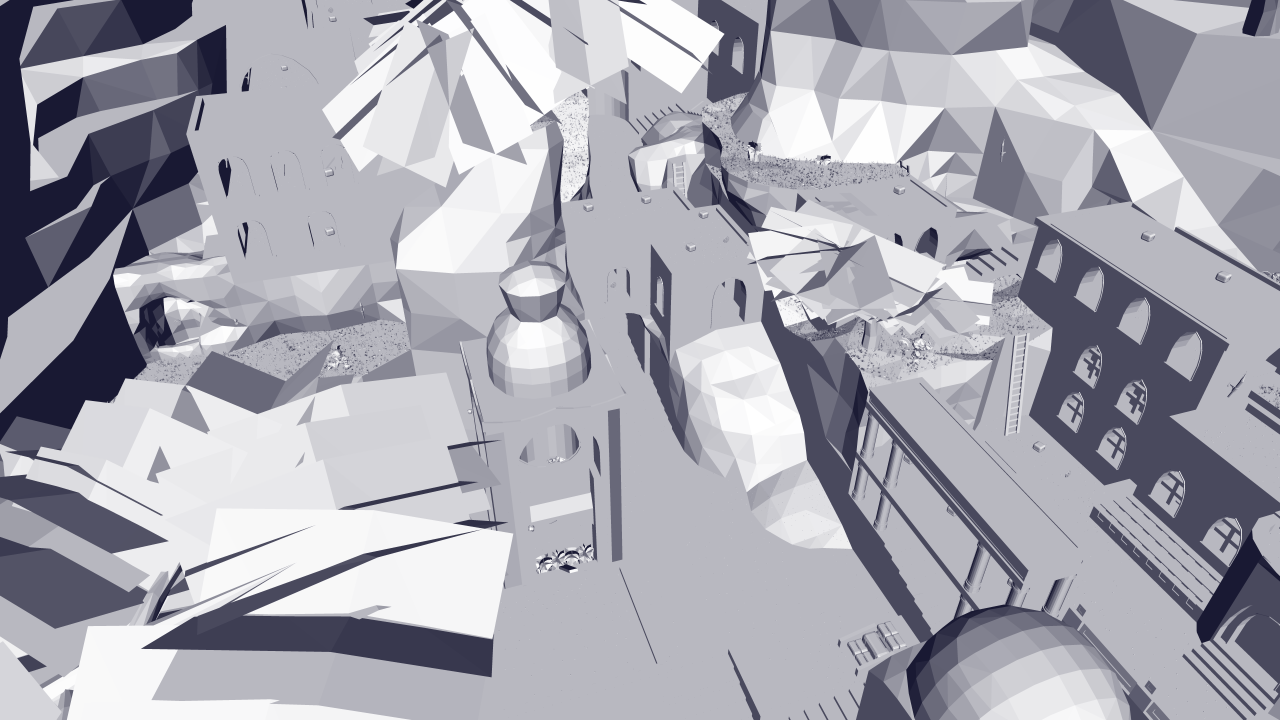
\includegraphics[width=\linewidth]{figures/eternal_valley_normal.png}
    \caption{Standard pipeline}
  \end{subfigure}\hfill
  \begin{subfigure}{0.48\textwidth}
    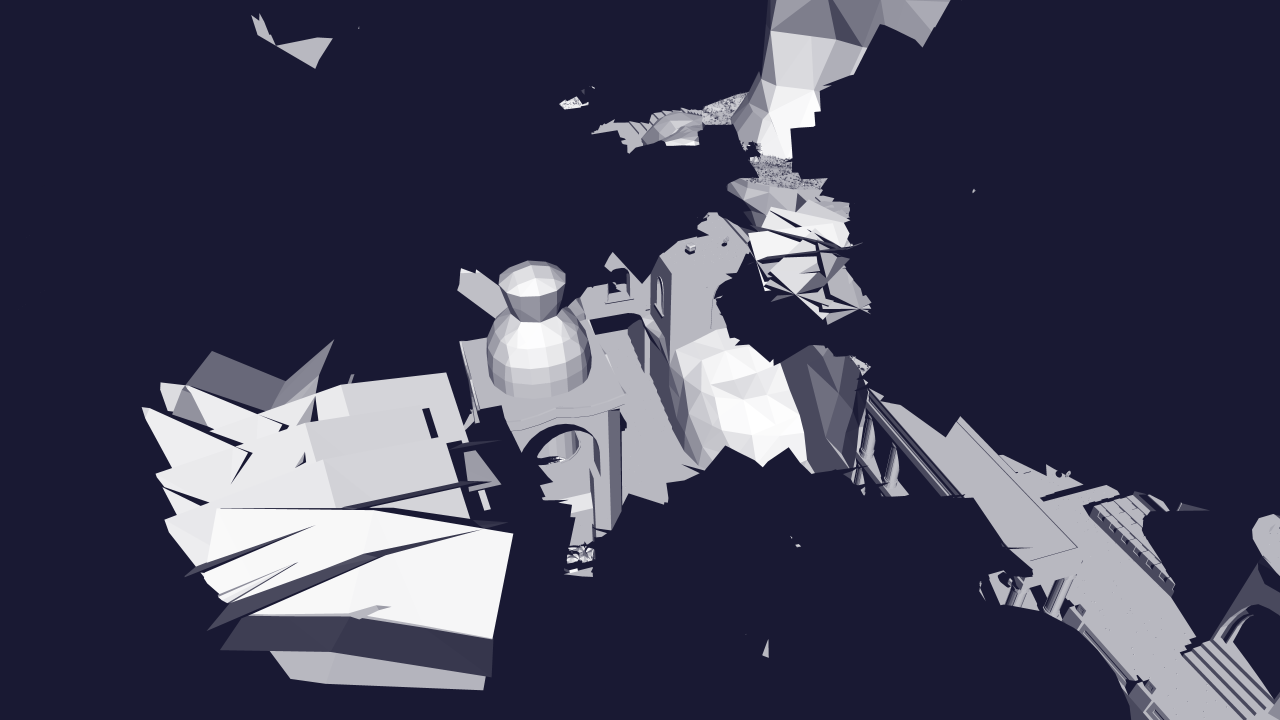
\includegraphics[width=\linewidth]{figures/eternal_valley_shadow.png}
    \caption{Shadow pipeline}
  \end{subfigure}

  \caption{Output images using different pipelines for the scene "Eternal Valley"}
\end{figure}\label{fig:eternal-valley}

\subsection{Performace}

We tested the different pipelines for the scene "Eternal Valley". We generated 64 frames with a resolution of $1280 \times 720$ pixels and 64 samples per pixel. We also rebuilt the acceleration structure every frame and preferred a fast trace for optimal ray tracing durations.

\begin{figure}[H]
  \centering
  % Left side: the image
  \begin{minipage}{0.6\textwidth}
    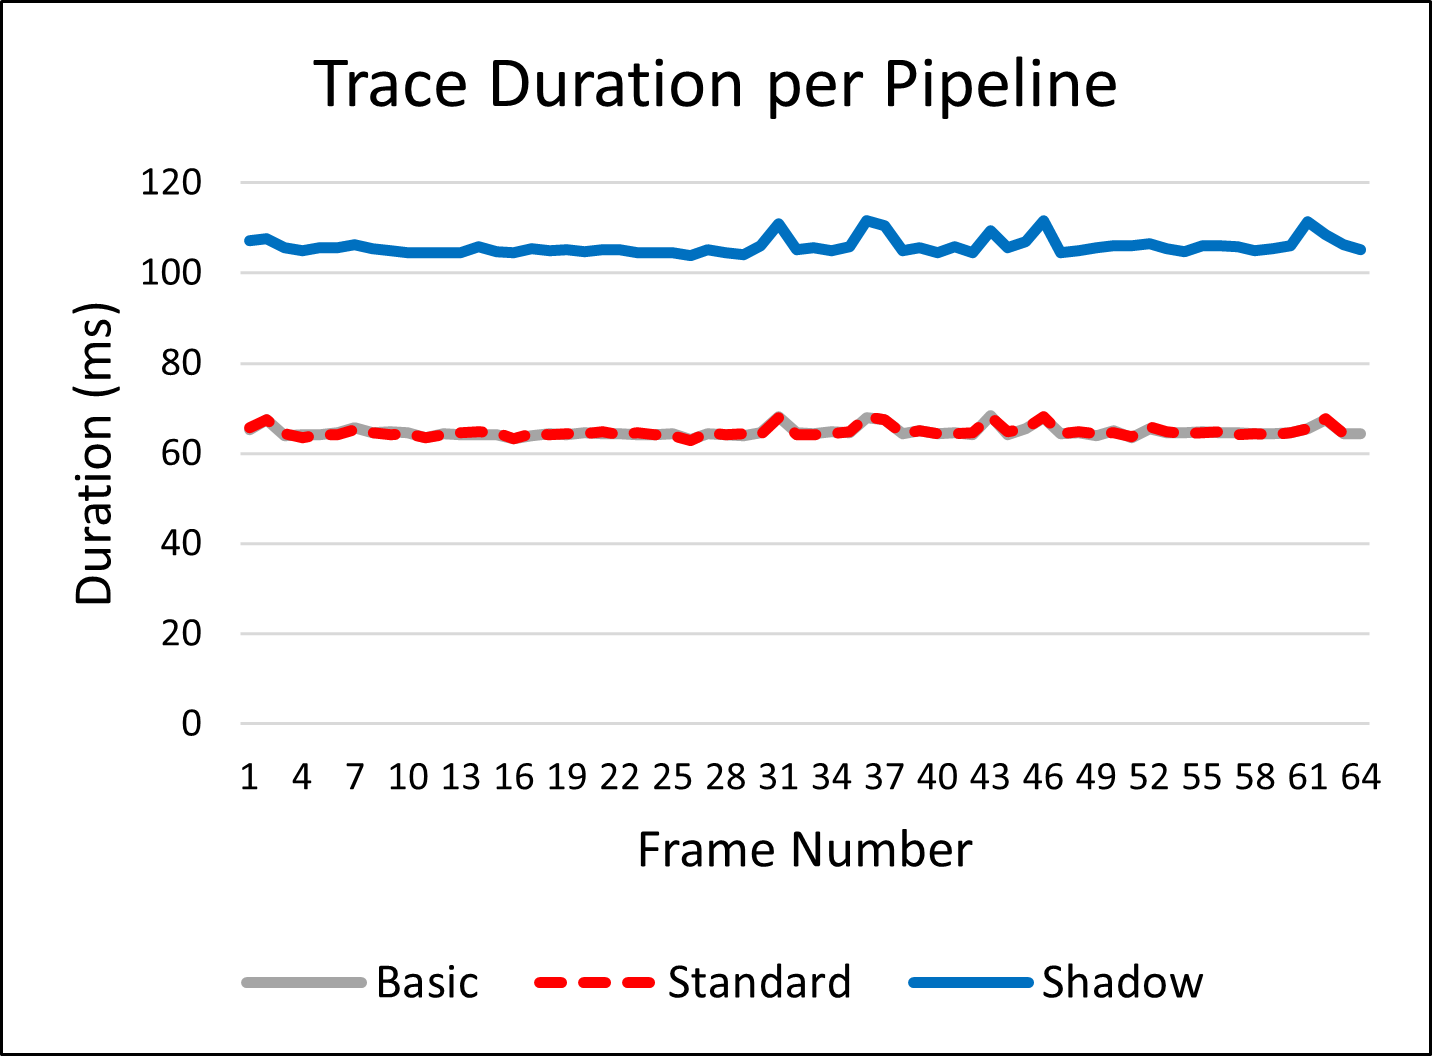
\includegraphics[width=\linewidth]{charts/pipeline.png}
    \caption{Impact of different pipelines on ray tracing duration}
  \end{minipage}\hfill
  % Right side: the table
  \begin{minipage}[t]{0.35\textwidth}
    \centering
    \begin{tabular}{|l|r|}
    \hline
    \textbf{Pipeline} &  \textbf{Avg. Trace} \\ \hline
    Basic             &  64.803 ms \\
    Standard          &  64.802 ms \\
    Shadow            & 105.898 ms \\ \hline
    \end{tabular}
    \captionof{table}{Average trace duration per pipeline}
  \end{minipage}
\end{figure}

The basic pipeline and standard pipeline have basically the same behaviour. This would mean that our shaders do not significantly impact the performance of our pipelines and that the large majority of time is spent on the traversal of the acceleration structure.

We can also see that our shadow pipeline takes up much more time than the other two. This makes sense because it casts an additional secondary ray for every primary ray that hits a surface. In our test scene, every ray hits a surface (see \autoref{fig:eternal-valley}), which means that every primary ray also produces a shadow ray, and the total number of rays in the shadow pipeline is double the number of rays in the other two pipelines. However, the trace duration only increases by about 63\% instead of 100\%. This has probably to do with the way we cast our shadow rays, because we use two flags that are not used for primary rays:

\begin{itemize}

  \item \code{gl\_RayFlagsSkipClosestHitShaderEXT}

  This flag prevents the ray from invoking the closest hit shader. We can use it because our implementation relies entirely on the miss shader. The surface point is assumed to be in shadow (\code{shadow = true}) and the miss shader then sets \code{shadow} to \code{false}.

  \item \code{gl\_RayFlagsTerminateOnFirstHitEXT}
   
  This flag terminates the traversal of the acceleration structure as soon as a ray hits anything. We only use the miss shader, which means that as soon as we hit something, the miss shader will not be invoked, and we can safely terminate early.

\end{itemize}

This could explain why shadow rays are cheaper in our implementation.

Another possible reason is that all shadow rays are parallel because we use a directional light source. This makes them more coherent and may also improve performance.

\section{Multi-Sampling}

\subsection{Output}

\begin{figure}[H]
  \centering

  \begin{subfigure}{0.3\textwidth}
    
\includegraphics[width=\linewidth]{figures/spp_1.png}
    \caption{1 spp}
  \end{subfigure}\hfill
  \begin{subfigure}{0.3\textwidth}
    
\includegraphics[width=\linewidth]{figures/spp_4.png}
    \caption{4 spp}
  \end{subfigure}\hfill
  \begin{subfigure}{0.3\textwidth}
    
\includegraphics[width=\linewidth]{figures/spp_16.png}
    \caption{16 spp}
  \end{subfigure}

  \caption{Comparison between images using a different number of samples per pixel}
\end{figure}

\subsection{Performace}

We tested different numbers of samples per pixel for the scene "Space Station" with the shadow pipeline. We generated 100 frames with a resolution of $1280 \times 720$ pixels. We also rebuilt the acceleration structure every frame and preferred a fast trace for optimal ray tracing durations.

\begin{figure}[H]
    \centering
    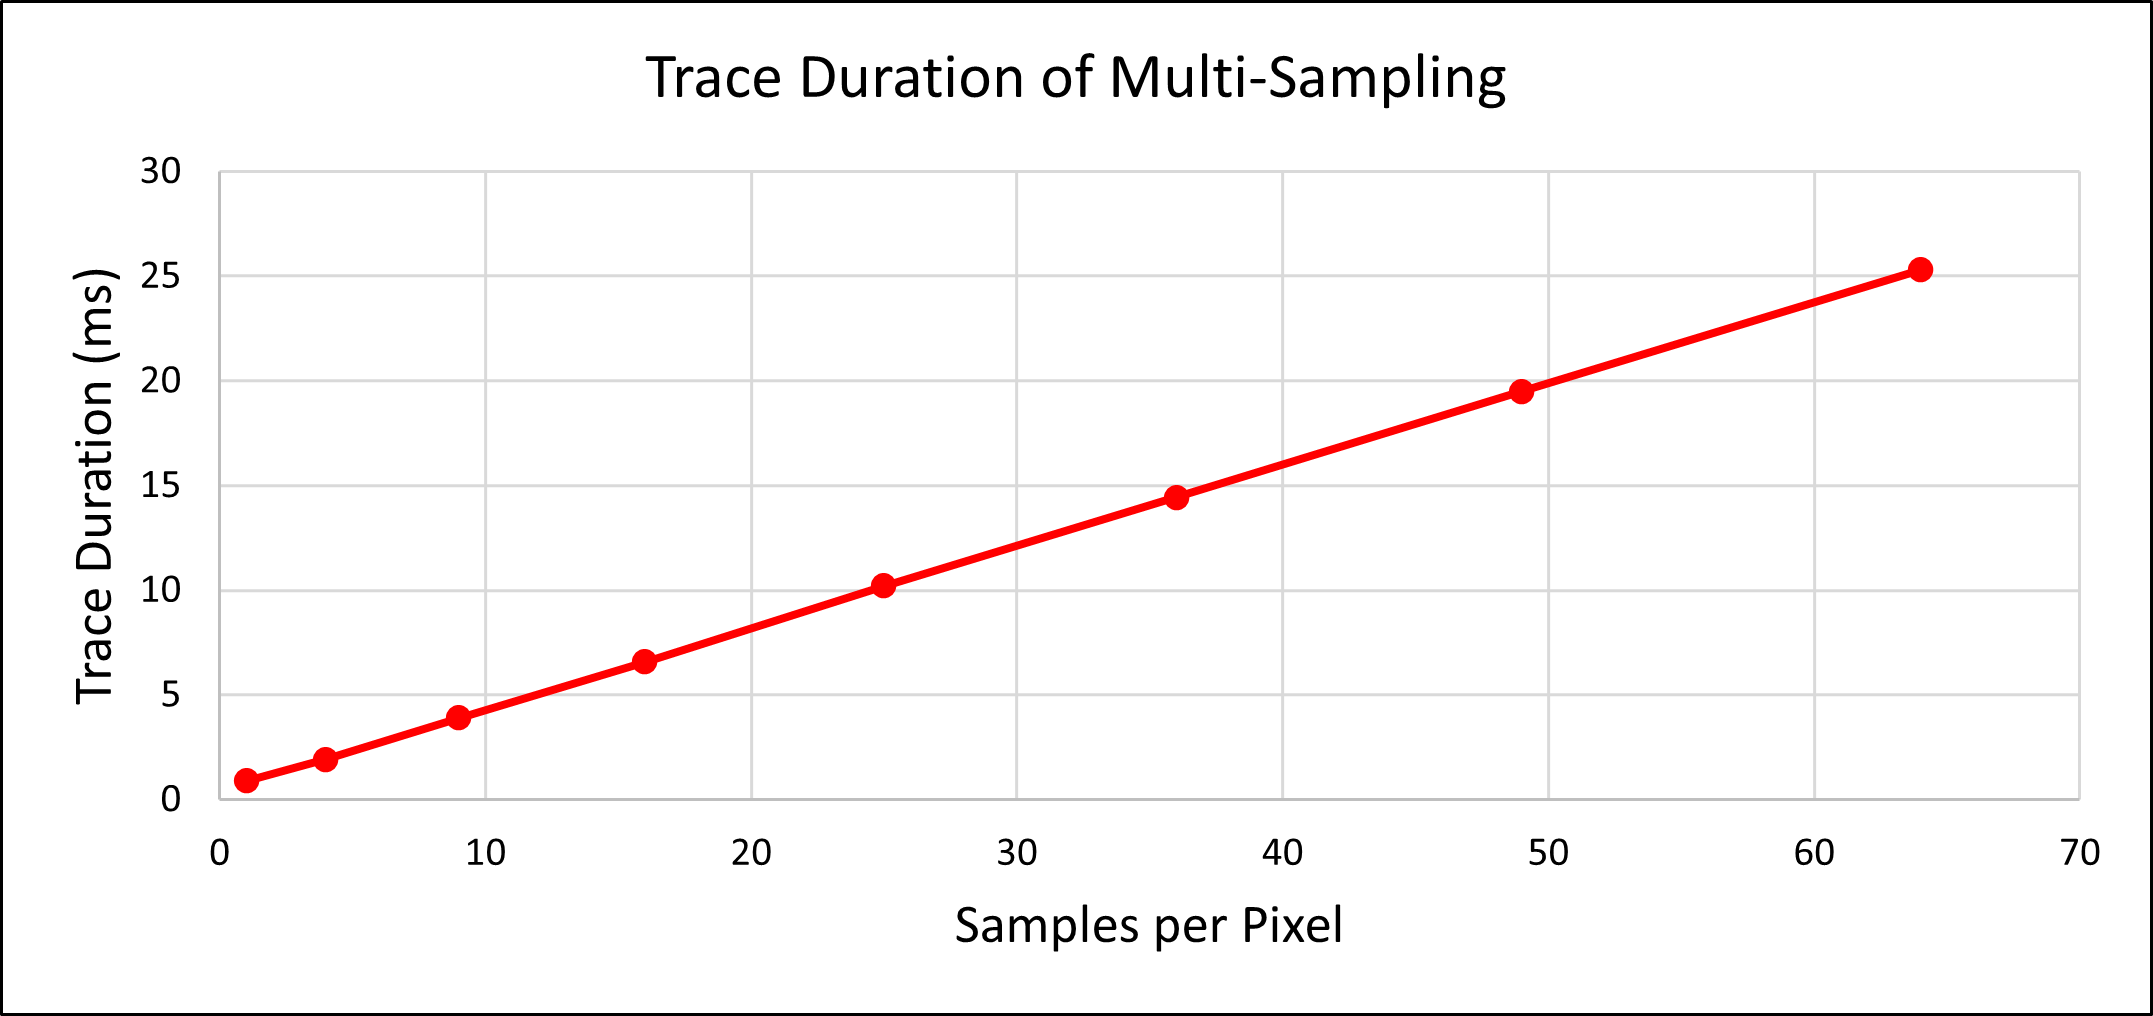
\includegraphics[width=0.9\textwidth]{charts/multi_sampling.png}
    \caption{Impact of multi-sampling on ray tracing duration}
\end{figure}

This chart shows that the duration of tracing the rays scales linearly with the number of samples per pixel. This makes sense because if we double the number of samples, we also double the number of rays. 

\section{Update Strategies}

We tested different strategies for updating the acceleration structure for the scene "Eternal Valley" with the standard pipeline. We generated 64 frames with a resolution of $1280 \times 720$ pixels and 64 samples per pixel and preferred a fast trace. We tested three strategies:

\begin{itemize}
  \item \textbf{Always Rebuild}: The acceleration structure gets completely rebuilt every frame.
  \item \textbf{Always Rrefit}: After initially building the acceleration, we only refit it every frame.
  \item \textbf{Rebuild Every Eight Frames}: We refit most frames, but we do a rebuild every eighth frame.
\end{itemize}

\begin{figure}[H]
  \centering

  \begin{subfigure}{0.48\textwidth}
    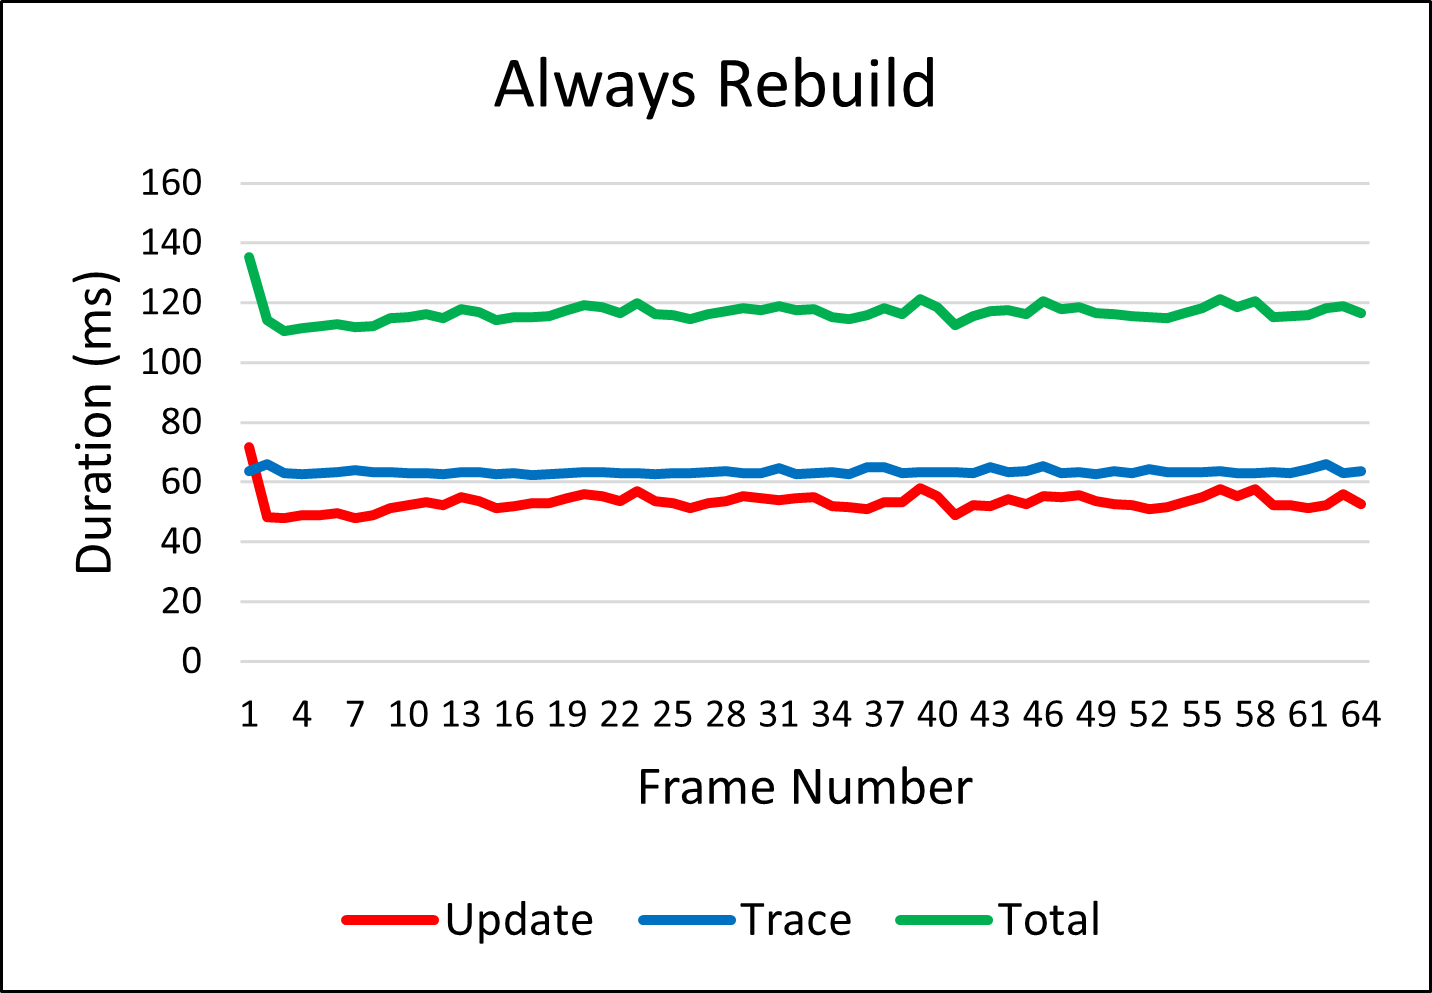
\includegraphics[width=\linewidth]{charts/always_rebuild.png}
    \caption{Always rebuild}
  \end{subfigure}\hfill
  \begin{subfigure}{0.48\textwidth}
    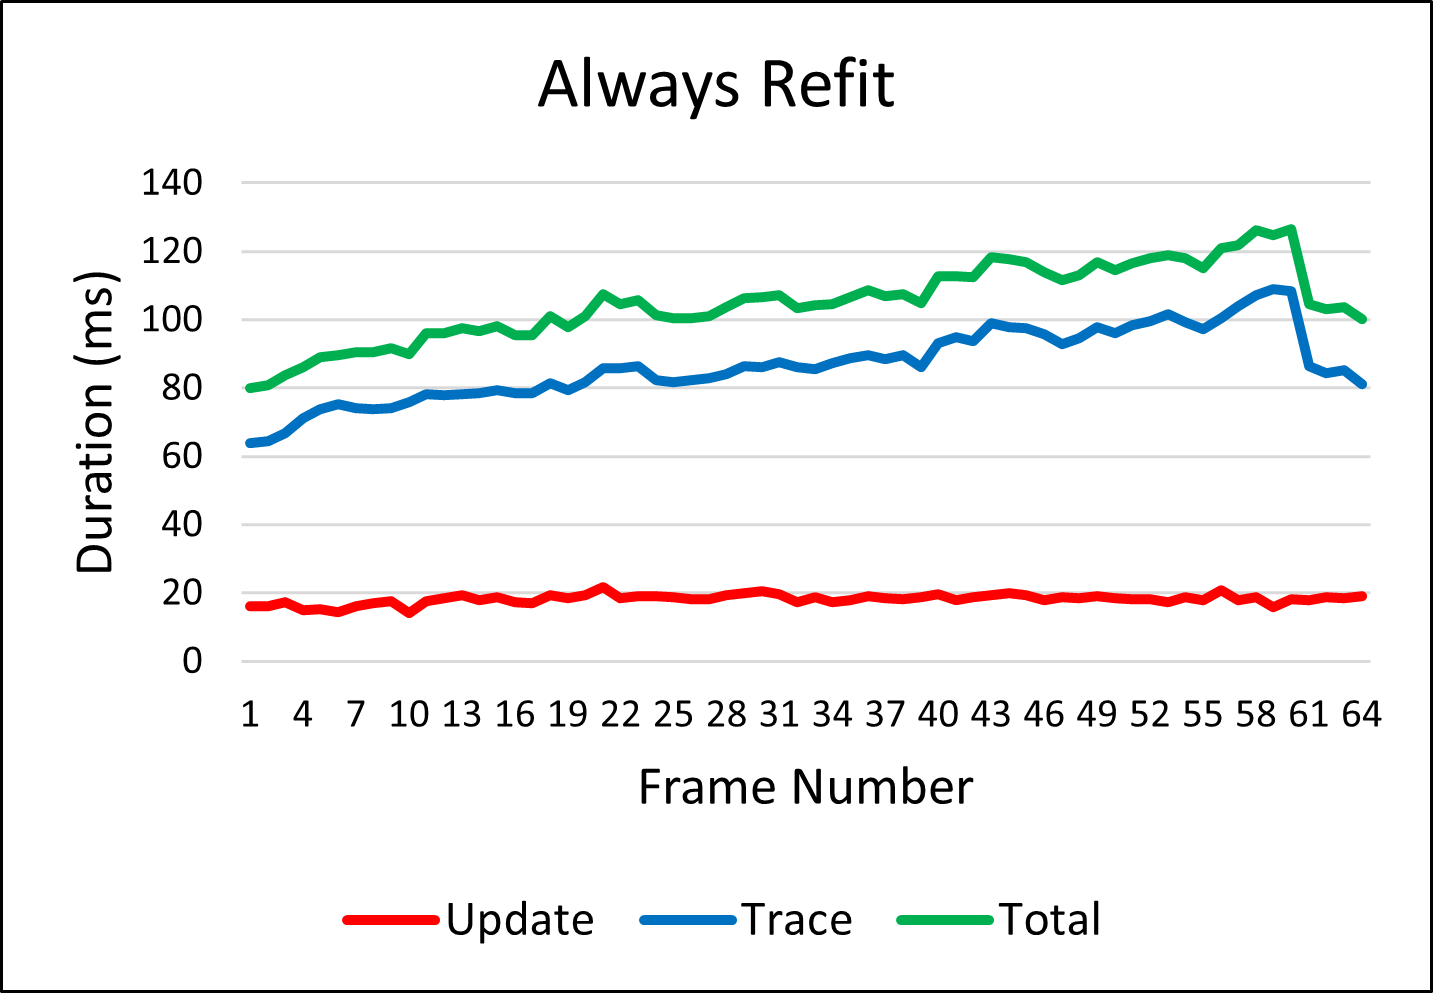
\includegraphics[width=\linewidth]{charts/always_refit.png}
    \caption{Always refit}
  \end{subfigure}\hfill
  \begin{subfigure}{0.72\textwidth}
    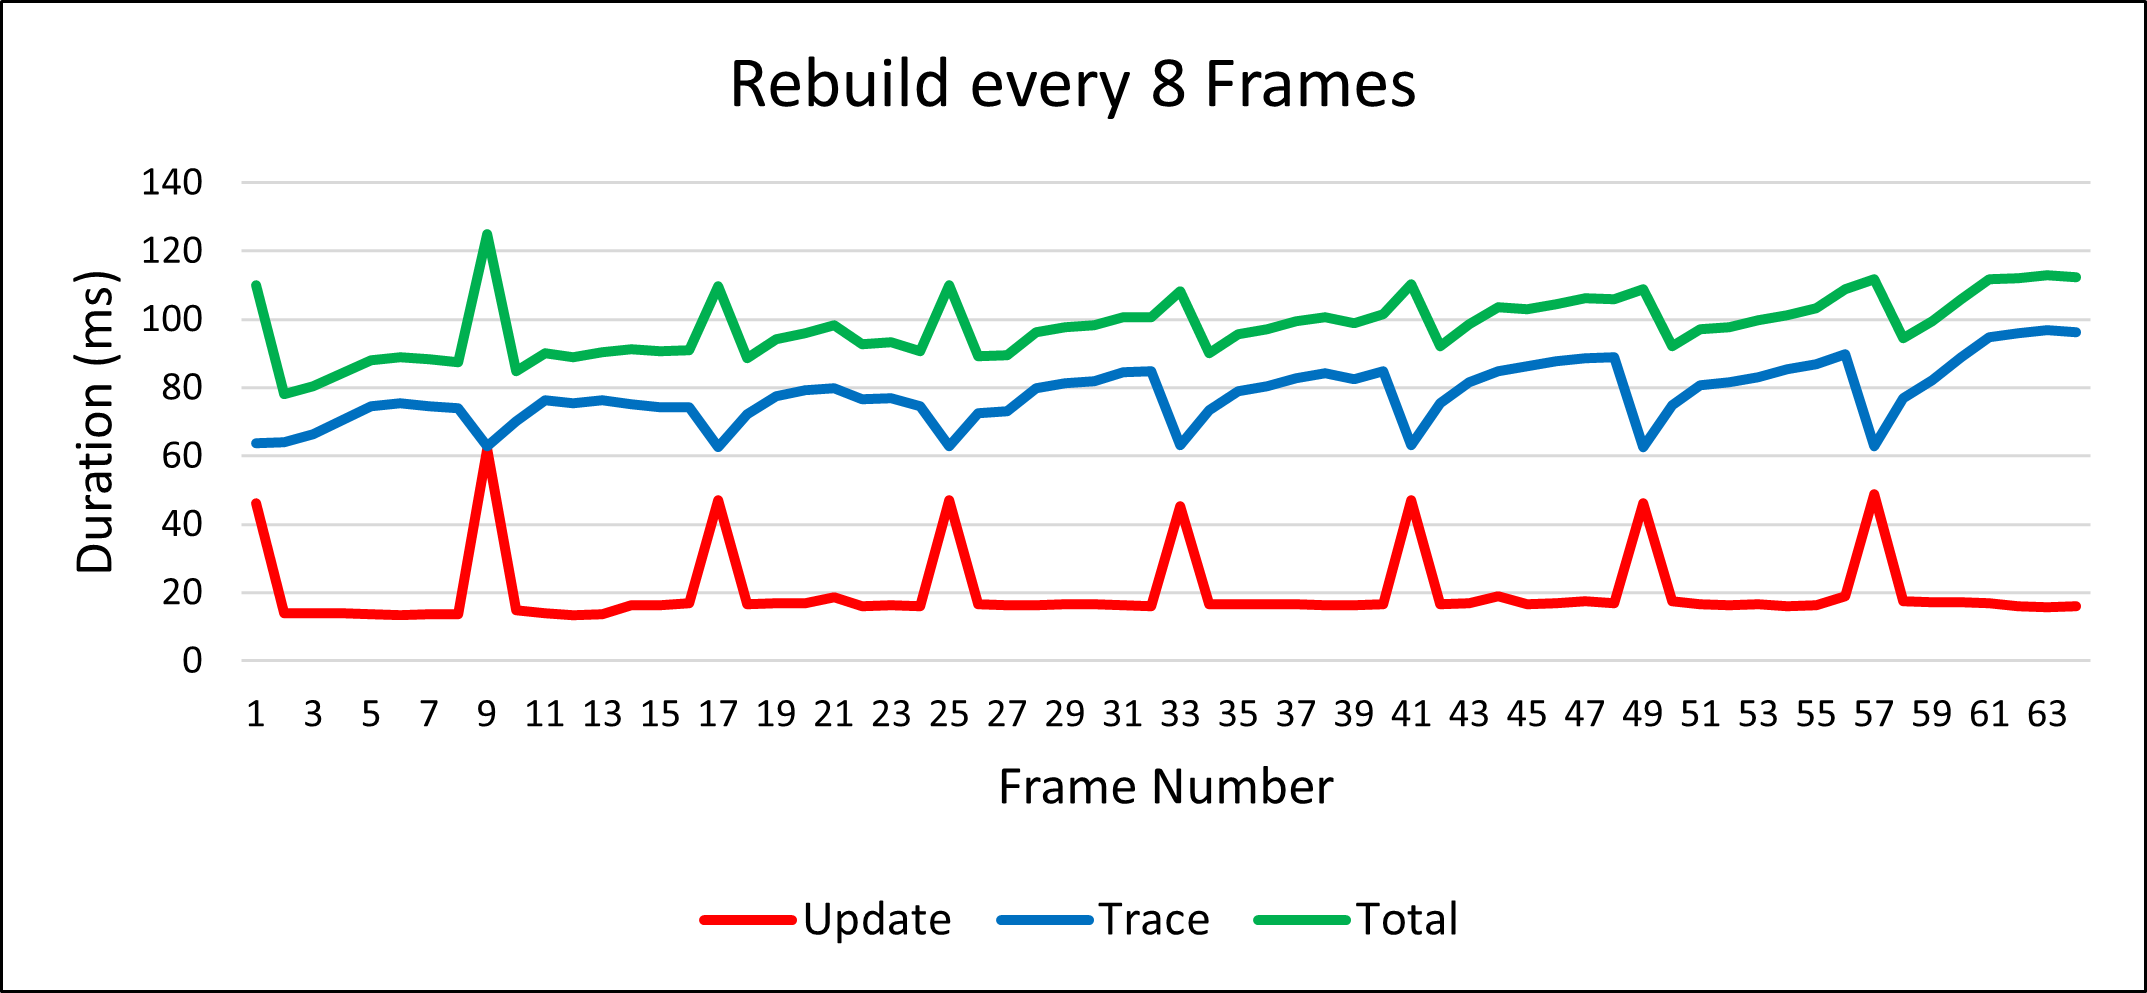
\includegraphics[width=\linewidth]{charts/rebuild_every_8_frames.png}
    \caption{Rebuild every eight frames}
  \end{subfigure}

  \caption{Comparing different strategies for updating the acceleration structure}
\end{figure}

\begin{figure}[H]
    \centering
    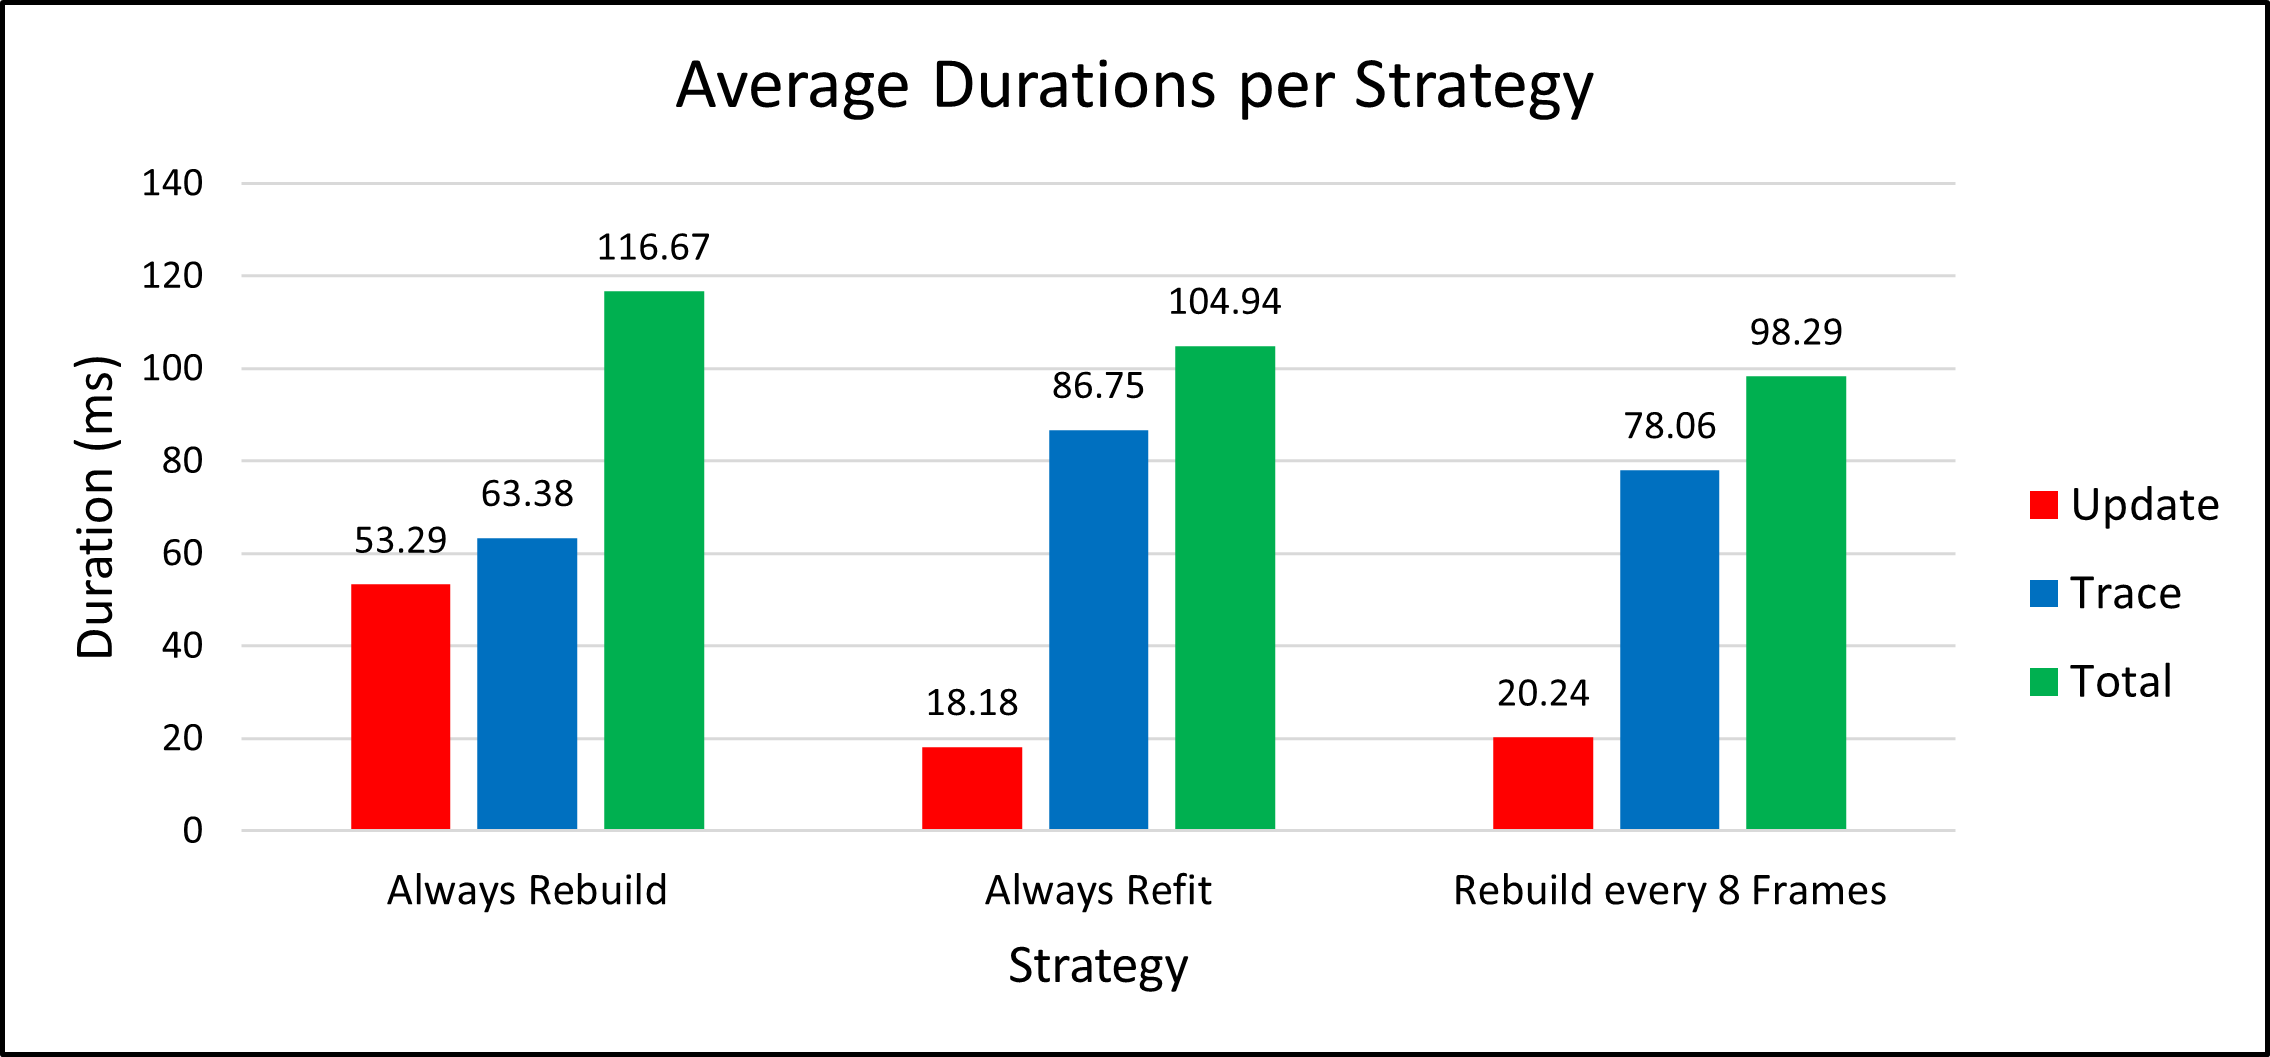
\includegraphics[width=0.9\textwidth]{charts/strategy_duration_avg.png}
    \caption{Comparing the average durations between different update strategies}
\end{figure}

\subsection{Always Rebuild}

As expected, always rebuilding gives us the shortest ray tracing duration, but it comes at the cost of a lot slower updates to the acceleration structure. The update and trace durations are very consistent; therefore, the total duration stays consistent. However, compared to the other strategies, it has the highest total duration on average.

\subsection{Always Refit}

This strategy results in very consistent and very short update durations. However, tracing the rays through the scenes becomes slower and slower, since the acceleration structure gets increasingly suboptimal. This causes the strategy to have a worse total time than always rebuilding towards the end of the animation. We can also notice that the trace duration suddenly decreases again at the end of the chart. The scene's animation is about 6 seconds long, and the delta time used was 0.1s. Thus, the animation finishes around frame 60 (shortly before the end of our chart) and starts to play again from the beginning. Since the BVH was also created at the beginning of the animation, refitting produces good results again.

\subsection{Rebuild Every Eight Frames}

This strategy is a mix of the previous two. The update duration is usually very short, but every eight frames it spikes due to a rebuild occuring, which also causes the trace duration drops at those points. After each rebuild, the trace duration rises again, but consistent rebuilds prevent it from diverging too far from the initial duration. This strategy has good average update and trace durations, which result in the best total duration on average compared to the other strategies.

\subsection{Discussion}

Because of the presented measurements, someone might assume that the third strategy is the best, but our measurements can not be generalized. If, for example, we keep increasing the number of rays, sooner or later, the strategy of always rebuilding will become more favorable. Always refitting, however, is rarely a good strategy. Even if not that many rays are traced, the BVH will become increasingly suboptimal in a lot of scenarios, which makes always refitting an unsustainable strategy. However, it might be viable for scenes that never change too much from their initial state.

\section{Fast Build vs. Fast Trace}

We tested the flags \code{PREFER\_FAST\_BUILD} and \code{PREFER\_FAST\_TRACE} for the scene "Eternal Valley" with the standard pipeline. We generated 50 frames with a resolution of $1280 \times 720$ pixels and 64 samples per pixel. We also rebuilt the acceleration structure for every frame since these flags do not affect refitting.

\begin{figure}[H]
  \centering

  \begin{subfigure}{0.48\textwidth}
    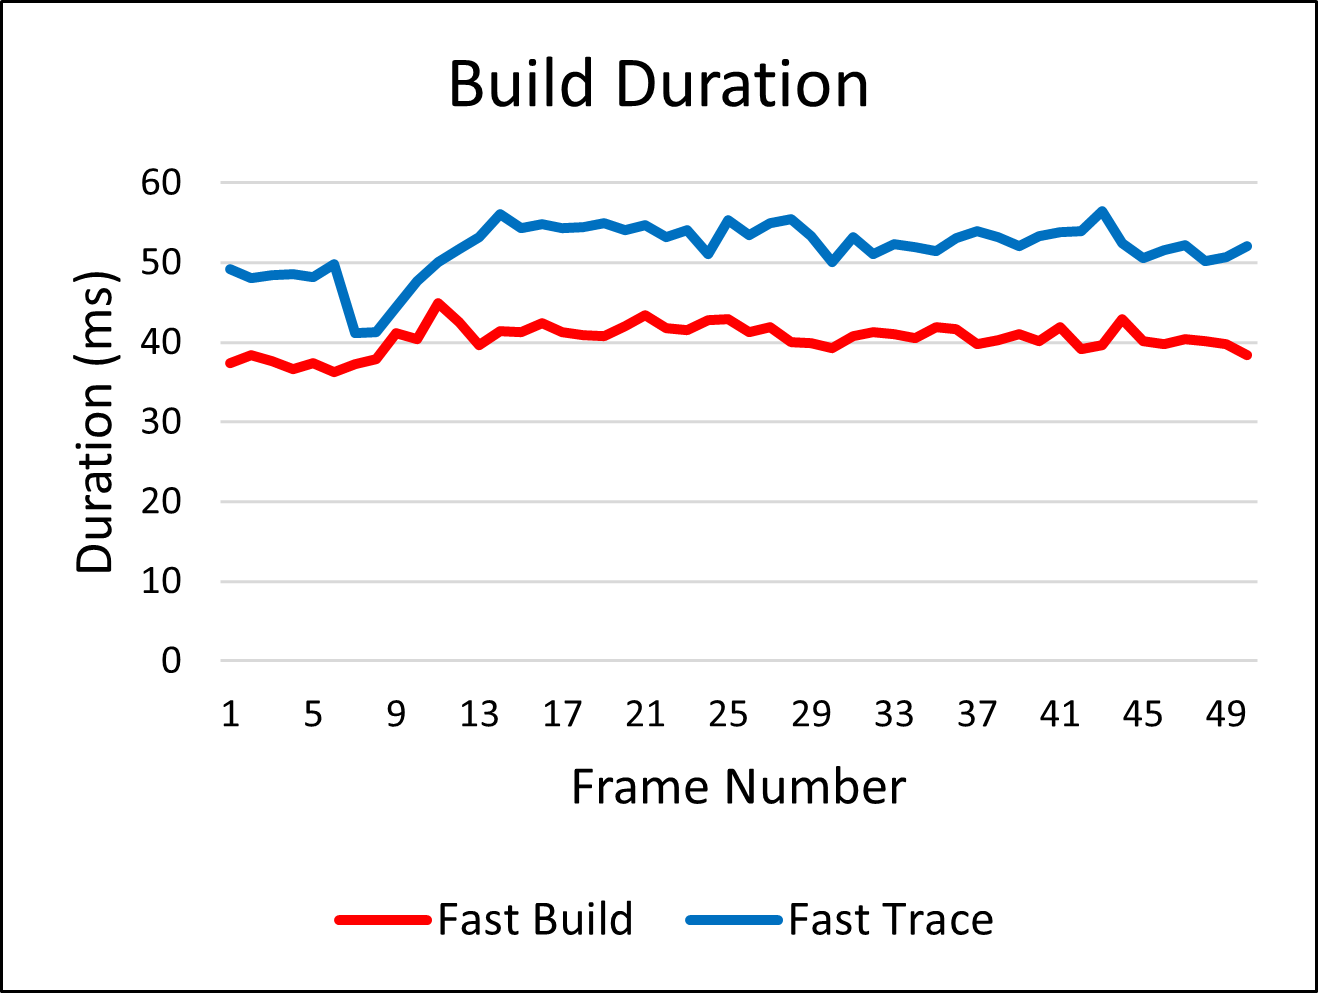
\includegraphics[width=\linewidth]{charts/fast_build_build.png}
    \caption{Build duration}
  \end{subfigure}\hfill
  \begin{subfigure}{0.48\textwidth}
    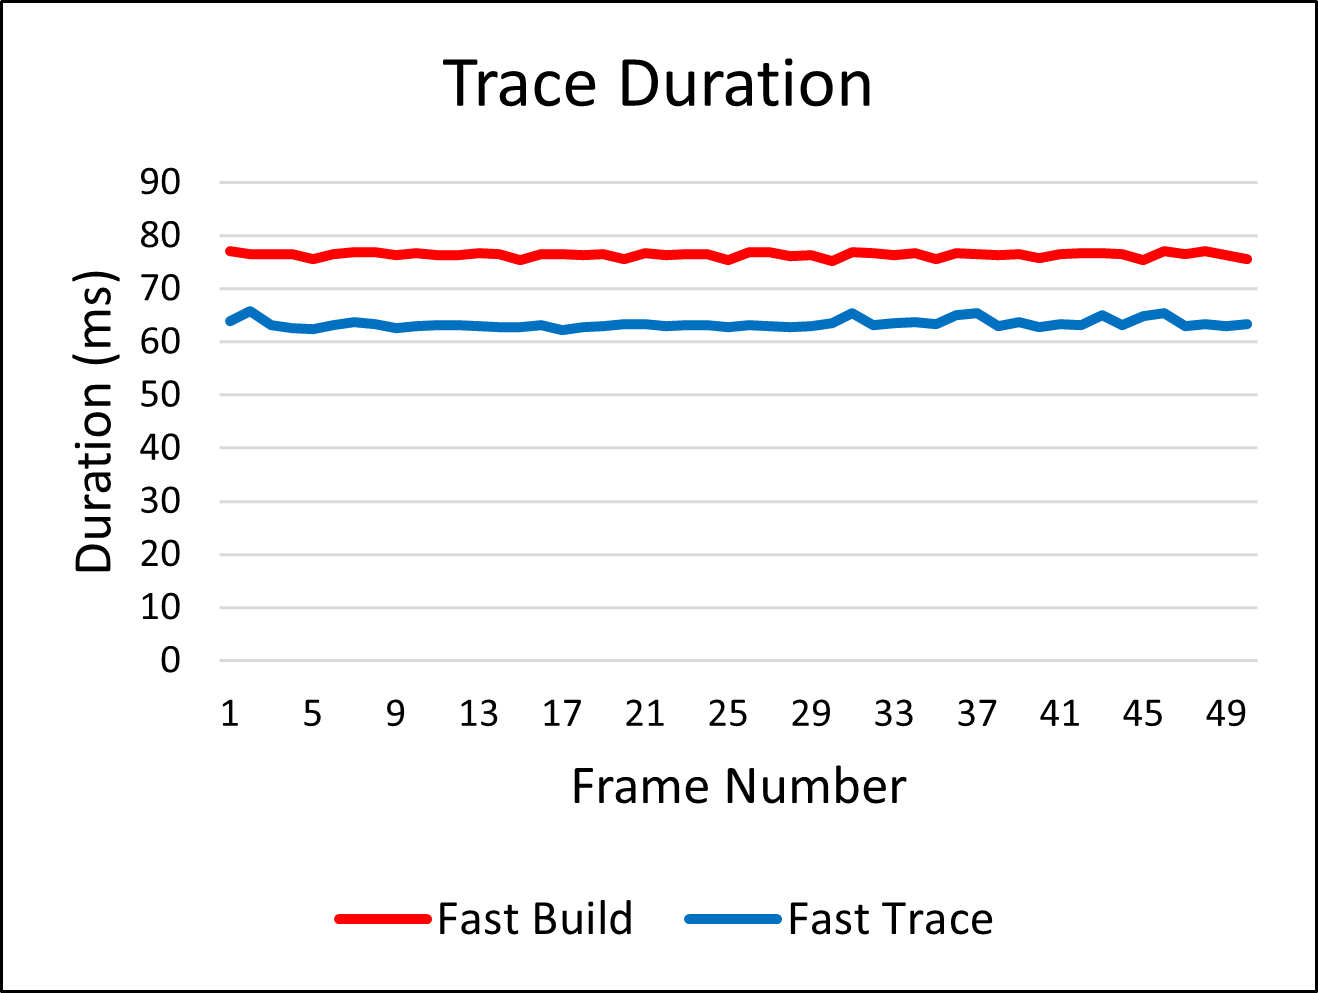
\includegraphics[width=\linewidth]{charts/fast_build_trace.png}
    \caption{Trace duration}
  \end{subfigure}

  \caption{Comparing the build and trace duration of the flag \code{PREFER\_FAST\_BUILD} to the flag \code{PREFER\_FAST\_TRACE}}.
\end{figure}

We can see the expected outcome of \code{PREFER\_FAST\_BUILD} having shorter build durations and longer trace durations compared to \code{PREFER\_FAST\_TRACE}. It is important to mention that these flags do not impact refitting. These flags only affect the structure of the BVH, which refitting does not touch.

Whether \code{PREFER\_FAST\_BUILD} or \code{PREFER\_FAST\_TRACE} should be used depends on the specific scenario. If many rays are traced and the trace duration is the bottleneck in the application, \code{PREFER\_FAST\_BUILD} should probably be used. On the other hand, if most of the time is spent on rebuilding (not refitting!), \code{PREFER\_FAST\_TRACE} is likely the better choice.